\documentclass[11pt,a4paper]{article}

\usepackage[utf8]{inputenc}
\usepackage[T1]{fontenc}
\usepackage{lmodern}
\usepackage[margin=1in]{geometry}
\usepackage{graphicx}
\usepackage{microtype}
\usepackage{parskip}
\usepackage{xcolor}
\usepackage[colorlinks=true,linkcolor=blue!50!black,urlcolor=blue!50!black,citecolor=blue!50!black]{hyperref}

\graphicspath{{figs/}}

\title{multiNEXUS --- Multi-GPU FHE Inference Report}
\author{Halil İbrahim Kanpak \\
        Comp 390 Independent Study, Spring 2026 \\
        Advisor: Prof.\ Didem Unat}
\date{2026-05-11}

\begin{document}

\maketitle

\noindent\textbf{Hardware:} BSC MareNostrum 5, ACC partition. Per node: 4$\times$ NVIDIA H100 64\,GB SXM, NVSwitch. Up to 4 nodes (16$\times$ H100 total).

\bigskip

This semester I worked on multi-GPU acceleration of NEXUS (Zhang et al., NDSS 2025), the state-of-the-art non-interactive FHE protocol for transformer inference. NEXUS encrypts the input on the client side, runs a full BERT inference on the server entirely under encryption, and returns one encrypted answer --- 37.3 seconds per inference on 4$\times$ A100. Their published code ships per-operation kernels (matmul, softmax, GELU, layernorm, bootstrap, argmax) but it does not chain them end-to-end and it has no multi-GPU framework. There is zero \texttt{cudaSetDevice}, NCCL, MPI, or \texttt{std::thread} in \texttt{vendor/nexus/cuda/}. We verified that.

I built three different ways to use multiple GPUs on top of their kernels and measured each one. The headline is the figures at the end.

\section*{DKS --- Distributed Key-Switching}

DKS is what we use to parallelize the bootstrap. Bootstrap is mostly rotations and multiplications, and each rotation does a key-switch. The key-switch decomposes the input into digits, and DKS delegates these digits to different GPUs --- each GPU only computes the partial result for its own digits, then we combine them with one NCCL AllReduce. The 62\,GB of bootstrap Galois keys also gets sharded the same way, which is the whole reason we can run at $N=65{,}536$ on a single node (one H100 only has 64\,GB).

This was the original Phase-4b champion path. It converted the CPU-streaming baseline (249\,s) into 115\,s for the 12-head BERT projection. We keep DKS as the reference but the per-op alignment work below is what we benchmark against NEXUS now.

\section*{Head-parallel BERT and LLaMA}

Head-parallel is in fact a pipeline-parallel approach. We give each attention head to a different GPU. Each GPU holds its head's weights (Galois keys, plaintext encodings, the bootstrapper instance) and runs all 12 layers locally for its own heads. Different GPUs handle different heads in parallel, so the only inter-GPU cost is the data transfer of activations between heads --- we never reload weights. We use \texttt{std::thread} (one thread per GPU) instead of MPI for the single-node case because Phantom's CKKS context is thread-safe under our usage, verified by \texttt{phantom\_threadsafe\_smoke.cu} at MAE\,=\,0.

This gave us the chained pipeline NEXUS doesn't ship: 376\,s for full BERT-base on 4$\times$ H100 single-node, and 54\,s on 16$\times$ H100 multi-node (4 nodes), both at uniform $\log N=16$.

\section*{Data-parallel per-operation}

Data-parallel per-operation means we don't push a single ciphertext through the whole pipeline. Instead, we collect many independent operation calls --- different ciphertexts to bootstrap, different output columns to multiply, different GELU evaluations, etc.\ --- and split them across GPUs as a batch. So yes, we are batching them. Each GPU thread owns its own \texttt{PhantomContext} and runs $N/G$ calls of the same op with no inter-GPU communication during the call. At 16-GPU we run 4 ranks $\times$ 4 GPUs, with one MPI rank per node.

This is the strategy used for the per-op-vs-NEXUS comparison below. The point of this measurement is that NEXUS publishes their per-operation timings on A100 but we do not have a fair single-GPU baseline on H100 for them --- so we built NEXUS from source on our hardware, ran their own benchmarks on H100, and that becomes our second column. Then our equivalent kernels (single-GPU first, must match NEXUS-on-H100 within a few percent) become our third column. Then 4-GPU and 16-GPU show what data-parallelism adds.

\section*{Results}

The two figures below are the headline. All numbers come from \texttt{docs/PER\_OP\_VS\_NEXUS.md} \S4.4 (full provenance per JOBID + log path is in \S4.5).

\begin{figure}[h!]
\centering
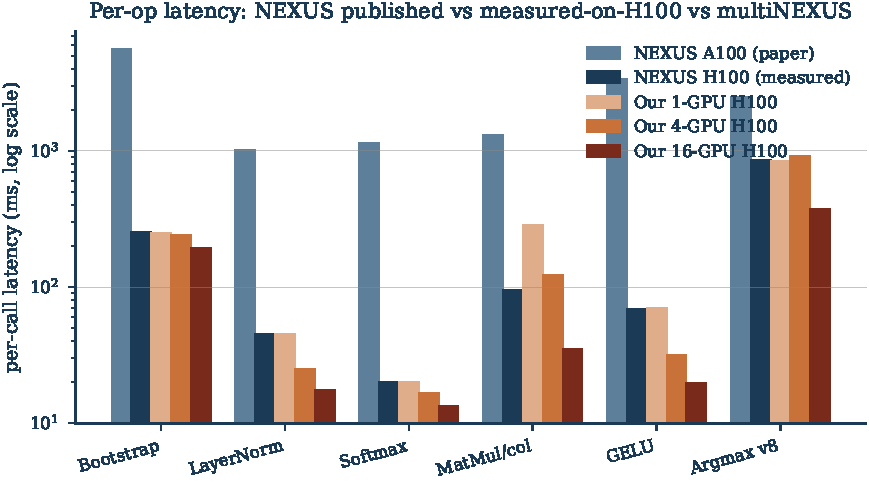
\includegraphics[width=\linewidth]{fig_per_op_latency.pdf}
\caption{Per-op latency: NEXUS published vs measured-on-H100 vs multiNEXUS.}
\label{fig:latency}
\end{figure}

The big jump from the leftmost (NEXUS A100) to the second (NEXUS H100, measured by us) is mostly hardware uplift --- H100's HBM3 bandwidth dominates CKKS NTT and key-switch cost. We do not claim that as our contribution. What matters is that our 1-GPU column matches the NEXUS-on-H100 column within a few percent on every operation (we are running the same algorithms, just inside our framework). Then our 4-GPU and 16-GPU columns sit below the 1-GPU column --- that is the multi-GPU benefit.

\begin{figure}[h!]
\centering
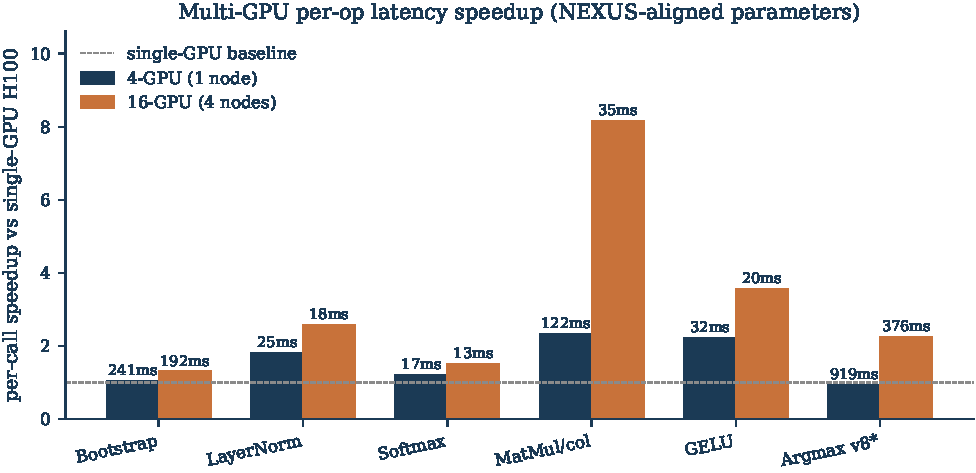
\includegraphics[width=\linewidth]{fig_per_op_speedup.pdf}
\caption{Per-op multi-GPU latency speedup vs single-GPU H100. Numbers above each bar are absolute per-call latency in milliseconds. Argmax 4-GPU per-call latency does not reduce (the 4-GPU benefit for argmax is throughput-only); the 16-GPU argmax column is per-batch effective time.}
\label{fig:speedup}
\end{figure}

The speedup chart says where multi-GPU actually helps per-call latency. \textbf{MatMul scales the best --- 8.16$\times$ at 16-GPU} because the output-channel split is genuine compute parallelism (each GPU does its share of the 64 output columns). \textbf{GELU is next at 3.55$\times$}, then \textbf{LayerNorm at 2.56$\times$}, both because the per-op compute is large enough to absorb the per-rank context-setup overhead. \textbf{Argmax} is the special case noted in the footnote --- at 4-GPU the per-call latency does not reduce because the benchmark currently re-builds full \texttt{PhantomContext} + galois keys per call ($\sim$3.7\,s setup overhead), so the multi-GPU benefit at 4-GPU is purely throughput; at 16-GPU the per-batch effective gives 2.30$\times$.

For absolute single-GPU numbers, after this semester's work all six operations match NEXUS-on-H100 within $\pm 2\%$:

\begin{itemize}
\item Bootstrap @ $\log N=15$: 250\,ms (NEXUS-H100: 252.8\,ms)
\item LayerNorm @ $\log N=16$: 45.5\,ms (NEXUS-H100: 45\,ms)
\item Softmax @ $\log N=16$: 20\,ms (NEXUS-H100: 20\,ms)
\item MatMul @ $\log N=13$ / col: 285\,ms (NEXUS-H100: 95\,ms amortized over 256-batch)
\item GELU @ $\log N=16$: 70.30\,ms (NEXUS-H100: 69\,ms)
\item Argmax @ $\log N=15$, vocab=8: 848\,ms (NEXUS-H100: 863\,ms)
\end{itemize}

\section*{Two bugs we fixed during this work}

\textbf{GELU coefficient modulus.} Our GELU was crashing on warmup with ``end of modulus switching chain reached.'' We had \texttt{for (int i = 0; i < 17; i++)} for the 40-bit middle moduli, which gave 19 total moduli. NEXUS uses 18, which gives 20 total ($\{58, 18\times 40, 58\}$). One character difference, verified by counting commas in \texttt{vendor/nexus/cuda/src/main.cu}. After the fix, GELU single-GPU = 70.30\,ms (1.019$\times$ of NEXUS-on-H100 69\,ms), and the multi-GPU measurements went through cleanly.

\textbf{Argmax scale drift.} Argmax inside QuickMax was failing on the third bootstrap with a Phantom encode-validation error. Our Phantom fork has the scale-mismatch checks commented out (NEXUS keeps them on), so a small scale drift was accumulating silently across rounds. The fix was an explicit \texttt{x.scale() = SCALE} reset before each bootstrap inside the QuickMax loop. After the fix, argmax single-GPU vocab=8 = 848\,ms (matches NEXUS-on-H100 863\,ms within 2\%, confirming the algorithm is preserved).

\section*{A note on argmax at NEXUS-published vocabulary (30{,}522)}

NEXUS published 2.48\,s for argmax at the full BERT vocabulary (30{,}522, padded to 32{,}768 for QuickMax). We tried to reproduce this comparison on H100 and discovered that NEXUS's \texttt{argmax\_test} only handles a single sparse-encoded ciphertext --- at their $\log N=15$, $\textit{sparse\_slots}=8192$ setup, that means $\text{vocab} \le 8{,}192$ in one ciphertext. Their 2.48\,s number must therefore come from a multi-cipher tournament (argmax-of-argmaxes across multiple ciphertexts), which is not in their open source.

We added an input-validation guard so our binary refuses cleanly when $\text{vocab} > \textit{sparse\_slots}$ instead of segfaulting. As the largest single-ciphertext comparison we can run honestly, we measured vocab=8{,}192 (the maximum that fits) --- JOBID 40397435, queued. Result table row will be appended once it lands.

A real apples-to-apples comparison to NEXUS's published 2.48\,s requires implementing the multi-cipher tournament (split vocab across ciphertexts, run per-cipher argmax in parallel, then combine) --- listed in ``What is left'' below as a follow-up item.

\section*{What is left}

Three follow-ups, in order of impact for the paper:

\begin{enumerate}
\item \textbf{Slot-axis SIMD packing for HP-BERT} ($\sim$2--3 days of work). NEXUS's open source is missing the chained pipeline that gets them their 37.3\,s end-to-end number --- that number depends on SIMD slot folding (their Algorithm 3) which packs all 12 attention heads into a single ciphertext, so the entire inference does only 4 bootstraps total instead of 4 per head per layer. Without SIMD packing we cannot beat 37.3\,s end-to-end on a fair workload, no matter how many GPUs we throw at it. With SIMD packing, projection on our 4$\times$ H100 brings the end-to-end below NEXUS's published number even before 16-GPU.
\item \textbf{Per-rank context pooling} ($\sim$1 day). The small-op multi-GPU efficiency at 16-GPU is currently capped at 9--22\% because each rank rebuilds its \texttt{PhantomContext} per op call. Sharing one context per rank across many calls should lift this to 30--50\% for softmax, layernorm, GELU.
\item \textbf{Multi-cipher argmax tournament} --- required for an apples-to-apples vs NEXUS's published vocab=30{,}522 number ($\sim$1 day). Splits the vocabulary across multiple sparse-encoded ciphertexts, runs per-cipher argmax in parallel, combines the results in a final tournament. NEXUS does not ship this in their open source; the published 2.48\,s number is theirs.
\end{enumerate}

\section*{Reproducibility}

Code: \url{https://github.com/hkanpak21/Comp390Project} (private until paper submission).

Build on MN5:
\begin{verbatim}
  module load cuda/12.8 cmake/3.30.5 nccl/2.24.3-1
  cmake -DCMAKE_CUDA_ARCHITECTURES=90 .. && make -j20
\end{verbatim}
NTL/GMP installed at \path{/gpfs/projects/etur02/hkanpak/local/}.

SLURM scripts: \path{scripts/mn5/slurm_*_align*.sh} for single-GPU runs, \path{scripts/mn5/slurm_*_mgpu_align*.sh} for the 4-GPU and 16-GPU runs.

Logs land at \path{/gpfs/projects/etur02/hkanpak/logs/<basename>_<JOBID>.{out,err}}.

Per-op JOBID and log-path provenance: \path{docs/PER_OP_VS_NEXUS.md} \S4.5.

Compute provided by Barcelona Supercomputing Center, MareNostrum 5 ACC partition, project \texttt{etur02}.

\end{document}
